\documentclass[10pt,a4paper]{article}
\usepackage[T1]{fontenc}
\usepackage[utf8]{inputenc}
\usepackage{lmodern,microtype}
\usepackage[a4paper,top=20mm,bottom=21mm,left=20mm,right=20mm,headheight=14pt]{geometry}
\usepackage{amsmath,amssymb,mathtools}
\usepackage{siunitx}
\DeclareSIUnit{\sample}{sample}
\sisetup{detect-all,group-separator={,},group-minimum-digits=4}
\usepackage{booktabs,tabularx,longtable,array}
\usepackage{enumitem}
\usepackage{xcolor}
\usepackage{tikz}
\usetikzlibrary{arrows.meta,positioning,calc,fit,backgrounds}
\usepackage{graphicx,caption}
\usepackage{fancyhdr,titlesec}
\usepackage{hyperref,bookmark}

\definecolor{navy}{HTML}{17324D}
\definecolor{blue}{HTML}{2563A6}
\definecolor{cyan}{HTML}{2E91A3}
\definecolor{green}{HTML}{3D7A57}
\definecolor{orange}{HTML}{C26A32}
\definecolor{lightblue}{HTML}{EAF2F8}
\definecolor{lightgray}{HTML}{F3F5F7}
\definecolor{linegray}{HTML}{AAB5C0}
\definecolor{textgray}{HTML}{465462}

\hypersetup{colorlinks=true,linkcolor=navy,urlcolor=blue,citecolor=blue,
  pdftitle={Bluetooth Channel Sounding Mode-0 Frequency Estimation and Phase Calibration},
  pdfauthor={Engineering report}}
\setlength{\parindent}{0pt}
\setlength{\parskip}{5.2pt}
\setlist{nosep,leftmargin=5.5mm}
\renewcommand{\arraystretch}{1.18}
\titleformat{\section}{\Large\bfseries\color{navy}}{\thesection}{0.6em}{}
\titleformat{\subsection}{\large\bfseries\color{navy}}{\thesubsection}{0.6em}{}
\titleformat{\subsubsection}{\normalsize\bfseries\color{navy}}{\thesubsubsection}{0.6em}{}
\captionsetup{font=small,labelfont={bf,color=navy}}
\pagestyle{fancy}
\fancyhf{}
\lhead{Bluetooth CS Mode-0 Frequency Estimation}
\rhead{Formal technical report - Revision 4.0}
\cfoot{\thepage}
\renewcommand{\headrulewidth}{0.4pt}

\newcommand{\code}[1]{\texttt{#1}}
\newcommand{\FFO}{\mathrm{FFO}}
\newcommand{\FAE}{\mathrm{FAE}}
\newcommand{\LFAE}{\mathrm{LFAE}}
\newcommand{\PCT}{\mathrm{PCT}}
\newcommand{\E}{\mathbb{E}}
\newcommand{\Var}{\operatorname{var}}
\newcommand{\argp}{\operatorname{Arg}}
\newcommand{\specbox}[1]{\begin{center}\fcolorbox{blue}{lightblue}{\parbox{0.92\linewidth}{#1}}\end{center}}
\newcommand{\implbox}[1]{\begin{center}\fcolorbox{green}{lightgray}{\parbox{0.92\linewidth}{#1}}\end{center}}

\begin{document}
\hypersetup{pageanchor=false}
\begin{titlepage}
\thispagestyle{empty}
\vspace*{13mm}
{\small\bfseries\color{blue} FORMAL TECHNICAL REPORT \hfill REVISION 4.0}\par
\vspace{25mm}
{\Huge\bfseries\color{navy} Bluetooth Channel Sounding\par}
\vspace{3mm}
{\Huge\bfseries\color{navy} Mode-0 Frequency Estimation\par}
\vspace{5mm}
{\Large\color{textgray} A self-contained derivation from oscillator coordinates and received I/Q samples to $f_{RX}[k]$, FFO, and PBR phase calibration}\par
\vspace{14mm}
\rule{\linewidth}{1.1pt}
\vspace{9mm}
{\large
This report defines every mathematical symbol and reference frame before use. It derives the received Mode-0 complex samples from the passband RF signal, derives two frequency estimators, reconstructs the Bluetooth quantity $f_{RX}[k]$, and substitutes that result into the exact FAE-adjusted fractional frequency offset equation. A numerical example demonstrates every intermediate value and sign. The separate Volume 1 reciprocal PCT phase-calibration and Inline PCT Transfer procedures are then connected to the Mode-0 frequency result.\par}
\vfill
\begin{tabular}{@{}ll@{}}
Primary references & Core 6.3, Vol. 1, Part A, Secs. 9.1-9.2; Vol. 6, Part A, Secs. 3.5 and 6.3\\
Air-interface timing & Core 6.3, Vol. 6, Part H, Secs. 4.3.1 and 4.6\\
Document type & Scientific and implementation-oriented technical report\\
Revision date & 4 September 2026
\end{tabular}
\end{titlepage}
\hypersetup{pageanchor=true}

\pagenumbering{roman}
\section*{Abstract}
Bluetooth Channel Sounding Mode-0 provides the relative frequency and timing calibration for the remaining steps of a CS subevent. The reflector transmits an \SI{80}{\micro\second} unmodulated tone; the initiator estimates its average frequency, denoted $f_{RX}[k]$, and combines it with the reflector's communicated Mode-0 frequency actuation error (FAE) to estimate fractional frequency offset (FFO). The specification defines the signal interval and the FFO quantities but does not prescribe a digital frequency estimator.

The central difficulty is reference-frame bookkeeping. A receiver does not observe RF frequency directly. It observes complex phase rotation relative to its own zero-baseband frequency and measures time with its own sample clock. This report establishes a receiver-local coordinate, defines local frequency actuation error (LFAE) as an error in that zero-baseband reference, derives the complex baseband model, and proves the reconstruction
\[
\widehat f_{RX}[k]=f_{c,cmd}^{(I)}[k]+\delta f_L^{(I)}[k]+s_{IQ}\widehat{\Delta f}_{BB}[k].
\]
Substitution into the Bluetooth FFO equation gives a direct expression from I/Q phase rate to $\widehat{\FFO}_{RX}[k]$. The report also derives the exact relative-oscillator interpretation, estimator ambiguity and variance, the complete \SI{2440}{\mega\hertz} example, and the distinct reciprocal PCT phase-calibration procedure from Volume 1, Part A, Sec. 9.2.

\specbox{\textbf{Normative boundary.} Bluetooth defines $f_{RX}[k]$ as the receiving device's estimate of the average received Mode-0 tone frequency, requires compensation of local actuation error, and defines the FAE-adjusted FFO equation. The RF architecture, I/Q convention, windowing, estimator, and quality gates are implementation choices and must be validated end to end.}

\tableofcontents
\clearpage
\pagenumbering{arabic}

\section{Scope and questions answered}
Mode-0 is not a distance measurement. It establishes the relative frequency and timing relationship that later RTT and PBR steps require. This report answers the following engineering questions.

\begin{enumerate}
\item Which part of the Mode-0 waveform is measured?
\item What exactly do $f_0[k]$, $f[k,1]$, $f_{RX}[k]$, FAE, LFAE, and FFO mean?
\item In whose frequency coordinate is $f_{RX}[k]$ expressed?
\item How does an RF sinusoid become $I[n]+jQ[n]$?
\item How does phase rotation in radians per sample become an RF-frequency estimate in hertz?
\item How is that estimate inserted into the Bluetooth FFO equation without double-counting FAE or LFAE?
\item How are several Mode-0 results combined, and how does the result interact with PBR phase calibration?
\end{enumerate}

The derivation assumes the initiator is the Mode-0 receiver and the reflector is the Mode-0 transmitter, matching the usual procedure. The equations remain valid with roles exchanged if all role labels and local calibrations are exchanged consistently.

\section{Normative map and calibration layers}
Core 6.3 Volume 1, Part A, Sec. 9.1 states that Mode-0 calibrates one device to the other in frequency and timing. Volume 6, Part H, Sec. 4.3.1 defines the Mode-0 packet and tone timing. Volume 6, Part A, Sec. 3.5.1 defines FFO and $f_{RX}[k]$. Volume 1, Part A, Sec. 9.2 separately defines reciprocal phase calibration for PBR.

\begin{longtable}{@{}p{0.28\linewidth}p{0.32\linewidth}p{0.33\linewidth}@{}}
\caption{Normative map.}\\
\toprule Source & Principal content & Use in this report \\
\midrule\endfirsthead
\toprule Source & Principal content & Use in this report \\
\midrule\endhead
Vol. 1, Part A, Sec. 9.1 & CS architecture and purpose of Modes 0-3 & Separates frequency/time calibration from RTT and PBR measurements.\\
Vol. 1, Part A, Sec. 9.2 & Reciprocal PCT equations and IPT architecture & Defines cancellation of relative LO phase.\\
Vol. 6, Part H, Sec. 4.3.1 & Mode-0 sequence, $T_{RD}$, $T_{IP1}$, $T_{GD}$, $T_{FM}$ & Defines the waveform interval used for frequency estimation.\\
Vol. 6, Part A, Sec. 3.5.1 & $f_0[k]$, $f[k,p]$, FAE, $f_{RX}[k]$, $\FFO_{RX}[k]$, $\FFO_{RX}^{*}$ & Provides the exact specification-level frequency quantities.\\
Vol. 6, Part A, Sec. 3.5.2 & Expected later transmitted frequencies & Connects Mode-0 with later CS steps.\\
Vol. 6, Part A, Secs. 6.3-6.5 & LFAE phase correction, PCT timing, IPT & Connects local actuation error and phase processing.\\
Vol. 6, Part H, Sec. 4.6 & PCT measurement period and exclusion regions & Defines samples valid for phase measurement.\\
RFPHY.TS, Sec. 4.8.1 & Instrument measurement of average Mode-0 tone frequency & Confirms the FAE-adjusted FFO calculation used for RF testing.\\
\bottomrule
\end{longtable}

\subsection{Three calibration layers}
\begin{tabularx}{\linewidth}{@{}p{0.20\linewidth}p{0.27\linewidth}X@{}}
\toprule Layer & Observable & Function \\
\midrule
Mode-0 frequency/time & $f_{RX}[k]$, $\FFO_{RX}[k]$, $\FFO_{RX}^{*}$ & Establishes the relative frequency scale; supports frequency placement and timing-scale compensation.\\
PBR phase/LO & $\PCT_{REFL}$ and $\PCT_{INIT}$, or IPT equivalent & Cancels relative LO phase and preserves twice the reciprocal channel phase.\\
Local RF implementation & LFAE, sample-rate, mixer sign, I/Q and RF-path corrections & Removes local deterministic errors not represented by the peer-to-peer equations.\\
\bottomrule
\end{tabularx}

\section{Mode-0 timing and measurement interval}
\subsection{Air-interface sequence}
The reflector's frequency-measurement tone follows its synchronization packet and guard interval. The fixed estimator-related durations are $T_{RD}=\SI{5}{\micro\second}$, $T_{GD}=\SI{10}{\micro\second}$, and $T_{FM}=\SI{80}{\micro\second}$. The configured $T_{IP1}$ lies in the allowed set 10, 20, 30, 40, 50, 60, 80, and \SI{145}{\micro\second}.

\begin{figure}[ht]
\centering
\resizebox{\linewidth}{!}{%
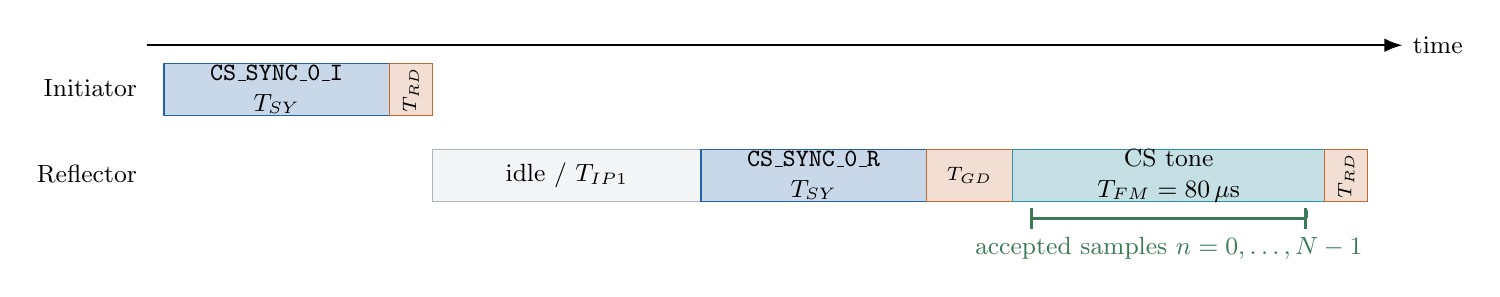
\begin{tikzpicture}[x=0.11cm,y=0.78cm,font=\small]
\draw[-Latex,thick] (0,2.7)--(145,2.7) node[right]{time};
\node[anchor=east] at (0,2.0) {Initiator};
\node[anchor=east] at (0,0.6) {Reflector};
\draw[fill=blue!25,draw=blue] (2,1.55) rectangle (28,2.4) node[midway,align=center]{\code{CS\_SYNC\_0\_I}\\$T_{SY}$};
\draw[fill=orange!22,draw=orange] (28,1.55) rectangle (33,2.4) node[midway,rotate=90]{\scriptsize $T_{RD}$};
\draw[fill=lightgray,draw=linegray] (33,0.15) rectangle (64,1.0) node[midway]{idle / $T_{IP1}$};
\draw[fill=blue!25,draw=blue] (64,0.15) rectangle (90,1.0) node[midway,align=center]{\code{CS\_SYNC\_0\_R}\\$T_{SY}$};
\draw[fill=orange!22,draw=orange] (90,0.15) rectangle (100,1.0) node[midway]{\scriptsize $T_{GD}$};
\draw[fill=cyan!28,draw=cyan] (100,0.15) rectangle (136,1.0) node[midway,align=center]{CS tone\\$T_{FM}=80\,\mu$s};
\draw[fill=orange!22,draw=orange] (136,0.15) rectangle (141,1.0) node[midway,rotate=90]{\scriptsize $T_{RD}$};
\draw[green,very thick,|-|] (102,-0.12)--(134,-0.12) node[midway,below=1mm]{accepted samples $n=0,\ldots,N-1$};
\draw[dashed,green] (102,-0.12)--(102,0.15); \draw[dashed,green] (134,-0.12)--(134,0.15);
\end{tikzpicture}}
\caption{Mode-0 timing. Frequency is estimated from the reflector's unmodulated CS tone during $T_{FM}$. Widths are labeled, not proportional.}
\label{fig:mode0time}
\end{figure}

Here $T_{SY}$ is the duration of the selected CS synchronization packet. The complete step duration is
\begin{equation}
T_{step,0}=2T_{SY}+2T_{RD}+T_{IP1}+T_{GD}+T_{FM}.
\end{equation}

\subsection{Implementation window}
Let $t_{FM,0}$ be the predicted start of the received tone in the initiator's local time coordinate. A receiver can select
\begin{equation}
W_k=[t_{FM,0}+t_{settle},\ t_{FM,0}+T_{FM}-t_{tail}],
\end{equation}
where $t_{settle}\ge0$ rejects front-end or NCO transients and $t_{tail}\ge0$ rejects ramp-down contamination. Define the accepted duration and sample count as
\begin{equation}
T_{obs}=T_{FM}-t_{settle}-t_{tail},\qquad N=\left\lfloor T_{obs}F_s\right\rfloor.
\end{equation}
Here $\lfloor x\rfloor$ is the greatest integer not exceeding $x$. The margins are implementation choices. Every reported estimate should retain $N$ and the actual window bounds.

\section{End-to-end processing overview}
Figure~\ref{fig:overview} gives the complete data dependency before the detailed derivation. No block can be omitted without changing the meaning of the result.

\begin{figure}[ht]
\centering
\resizebox{\linewidth}{!}{%
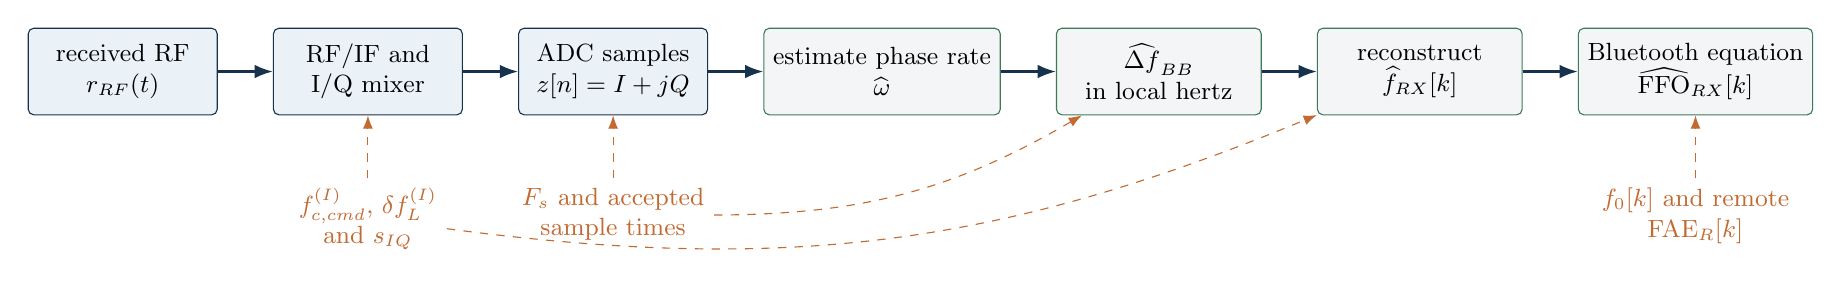
\begin{tikzpicture}[font=\small,>=Latex,node distance=7mm]
\tikzset{b/.style={draw=navy,rounded corners=2pt,fill=lightblue,minimum width=24mm,minimum height=11mm,align=center}, c/.style={draw=green,rounded corners=2pt,fill=lightgray,minimum width=26mm,minimum height=11mm,align=center}, a/.style={-Latex,thick,color=navy}}
\node[b] (rf) {received RF\\$r_{RF}(t)$};
\node[b,right=of rf] (mix) {RF/IF and\\I/Q mixer};
\node[b,right=of mix] (adc) {ADC samples\\$z[n]=I+jQ$};
\node[c,right=of adc] (phase) {estimate phase rate\\$\widehat\omega$};
\node[c,right=of phase] (bb) {$\widehat{\Delta f}_{BB}$\\in local hertz};
\node[c,right=of bb] (recon) {reconstruct\\$\widehat f_{RX}[k]$};
\node[c,right=of recon] (ffo) {Bluetooth equation\\$\widehat\FFO_{RX}[k]$};
\draw[a] (rf)--(mix);\draw[a] (mix)--(adc);\draw[a] (adc)--(phase);\draw[a] (phase)--(bb);\draw[a] (bb)--(recon);\draw[a] (recon)--(ffo);
\node[below=8mm of mix,align=center,text=orange] (zero) {$f_{c,cmd}^{(I)}$, $\delta f_L^{(I)}$\\and $s_{IQ}$};
\node[below=8mm of adc,align=center,text=orange] (clock) {$F_s$ and accepted\\sample times};
\node[below=8mm of ffo,align=center,text=orange] (remote) {$f_0[k]$ and remote\\$\FAE_R[k]$};
\draw[-Latex,dashed,orange] (zero)--(mix);\draw[-Latex,dashed,orange] (zero) to[bend right=15] (recon);\draw[-Latex,dashed,orange] (clock)--(adc);\draw[-Latex,dashed,orange] (clock) to[bend right=15] (bb);\draw[-Latex,dashed,orange] (remote)--(ffo);
\end{tikzpicture}}
\caption{End-to-end Mode-0 measurement chain. Superscript $(I)$ means a quantity expressed in the initiator's calibrated local coordinate.}
\label{fig:overview}
\end{figure}

\clearpage
\section{Mathematical framework and complete symbol definitions}
\label{sec:framework}
This section fixes the reference frame, dimensions, and sign convention used in Sections 6-8. Symbols are not used before they are defined.

\subsection{Indices, devices, and time coordinates}
\begin{itemize}
\item $M$ is the number of Mode-0 steps at the start of the subevent, and $k\in\{1,\ldots,M\}$ is a Mode-0 step index.
\item $R$ denotes the reflector, which transmits the measured Mode-0 tone.
\item $I$ denotes the initiator, which receives the tone and computes FFO.
\item $t$ is an ideal physical time coordinate used only to derive the relative-oscillator interpretation.
\item $\tau_I$ is the initiator-local calibrated time coordinate used by the receiver implementation.
\item $n\in\{0,\ldots,N-1\}$ is a complex-sample index and $\tau_n=nT_s$.
\item $F_s$ is the calibrated complex sample rate in samples per initiator-local second; $T_s=1/F_s$.
\end{itemize}

Let the initiator clock scale be $1+\epsilon_I$ relative to ideal time:
\begin{equation}
\tau_I=(1+\epsilon_I)t.
\label{eq:localtime}
\end{equation}
If a physical sinusoid is $e^{j2\pi f^{(phys)}t}$, then in initiator time
\begin{equation}
e^{j2\pi f^{(phys)}t}=e^{j2\pi f^{(I)}\tau_I},\qquad
f^{(I)}\equiv\frac{f^{(phys)}}{1+\epsilon_I}.
\label{eq:freqcoordinate}
\end{equation}
Thus a superscript $(I)$ means ``numerical frequency measured per initiator-local second.'' This is the natural coordinate of its LO, sample clock, timestamps, and digital estimator.
For samples generated by the same local timebase, $\tau_n=n/F_s$ and the corresponding ideal physical time is $t_n=n/[F_s(1+\epsilon_I)]$.

\subsection{Protocol frequencies and dimensionless errors}
\begin{longtable}{@{}p{0.22\linewidth}p{0.60\linewidth}p{0.10\linewidth}@{}}
\caption{Frequency and error symbols.}\\
\toprule Symbol & Definition & Unit \\
\midrule\endfirsthead
\toprule Symbol & Definition & Unit \\
\midrule\endhead
$f_0[k]$ & Nominal center frequency assigned to the CS channel in step $k$. & Hz\\
$f_R^{tx,phys}[k]$ & Actual average physical RF frequency transmitted by the reflector during the Mode-0 tone. & Hz\\
$f_{RX}^{(I)}[k]$ & Average received tone frequency expressed in the initiator-local coordinate after local calibration; this is the implementation realization of the specification's $f_{RX}[k]$. & Hz\\
$a_R[k]$ & Dimensionless reflector FAE, $a_R[k]=10^{-6}\FAE_R[k]$. & 1\\
$\eta_{R/I}[k]$ & Dimensionless remote-to-local fractional frequency offset, $\eta_{R/I}=10^{-6}\FFO_{R/I}$. & 1\\
$f_{ref,R}[k]$ & FAE-adjusted reflector reference, $f_0[k](1+a_R[k])$. & Hz\\
$f_{c,cmd}^{(I)}[k]$ & Receiver command frequency that would map to zero complex-baseband frequency if local actuation were perfect. It includes any declared analog LO and digital NCO translation. & Hz\\
$\delta f_L^{(I)}[k]$ & Local zero-baseband frequency error: actual calibrated zero-baseband reference minus commanded zero-baseband reference. Positive means the actual zero is above the command. & Hz\\
$f_c^{(I)}[k]$ & Actual calibrated zero-baseband reference, $f_{c,cmd}^{(I)}[k]+\delta f_L^{(I)}[k]$. & Hz\\
$\lambda_I[k]$ & Dimensionless local actuation error under this sign convention; $\delta f_L^{(I)}=f_{c,cmd}^{(I)}\lambda_I$. If stored in ppm, $\lambda_I=10^{-6}\LFAE_I$. & 1\\
$\Delta f_{BB}[k]$ & Signed rotation frequency of the accepted complex baseband tone. & Hz\\
$s_{IQ}$ & I/Q orientation sign, $+1$ or $-1$, defined by Eq.~\ref{eq:bbdef}. & 1\\
\bottomrule
\end{longtable}

\subsection{Complex-sample and estimator symbols}
\begin{longtable}{@{}p{0.22\linewidth}p{0.60\linewidth}p{0.10\linewidth}@{}}
\caption{Signal-processing symbols.}\\
\toprule Symbol & Definition & Unit \\
\midrule\endfirsthead
\toprule Symbol & Definition & Unit \\
\midrule\endhead
$z[n]=I[n]+jQ[n]$ & Accepted complex baseband sample. & ADC units\\
$I[n],Q[n]$ & Real in-phase and quadrature ADC components. & ADC units\\
$j$ & Imaginary unit, $j^2=-1$. & 1\\
$\rho[n]$ & Nonnegative desired-tone magnitude at sample $n$. & ADC units\\
$\phi_0$ & Constant received phase at the start of the accepted window. & rad\\
$\psi[n]$ & Residual time-varying phase from phase noise, motion, or channel evolution. & rad\\
$d[n]$ & Complex DC/LO-leakage component. & ADC units\\
$v[n]$ & Additive complex noise and interference. & ADC units\\
$\omega$ & Desired mean discrete-time phase increment, $2\pi\Delta f_{BB}/F_s$. & rad/sample\\
$m$ & Positive integer correlation lag. & samples\\
$w_n$ & Nonnegative estimator weight. & 1\\
$R_m$ & Weighted lag-$m$ complex correlation. & ADC units squared\\
$\argp(\cdot)$ & Principal argument in $(-\pi,\pi]$. & rad\\
$\E[\cdot]$ & Statistical expectation operator. & varies\\
$\Var(\cdot)$ & Statistical variance operator. & squared units\\
$q$ & Integer alias index used to unwrap $m\omega$. & 1\\
$\widehat{x}$ & Estimate of quantity $x$. & same as $x$\\
\bottomrule
\end{longtable}

\subsection{I/Q sign convention}
The report defines $s_{IQ}$ through
\begin{equation}
\Delta f_{BB}[k]=s_{IQ}\left(f_{RX}^{(I)}[k]-f_c^{(I)}[k]\right),
\qquad s_{IQ}\in\{+1,-1\}.
\label{eq:bbdef}
\end{equation}
For the common convention in which an RF tone above the zero-baseband reference rotates counterclockwise, $s_{IQ}=+1$. Swapping I and Q, conjugating samples, or using the opposite complex mixer changes the sign. Because $s_{IQ}^{-1}=s_{IQ}$, inversion gives
\begin{equation}
f_{RX}^{(I)}[k]=f_c^{(I)}[k]+s_{IQ}\Delta f_{BB}[k].
\label{eq:bbinvert}
\end{equation}

\subsection{Assumptions used for derivations}
The exact Bluetooth FFO definitions do not require these assumptions. The I/Q estimator derivations assume: (i) the accepted tone is dominated by one narrowband component; (ii) $F_s$ is known in the initiator coordinate; (iii) the desired phase is approximately affine over $T_{obs}$; (iv) weights are real and nonnegative; and (v) the acquisition stage resolves correlation aliases. Departures from these assumptions are treated as error sources, not hidden inside undefined terms.

\clearpage
\section{Exact FFO equations and oscillator-frame derivation}
\label{sec:ffoderivation}
\subsection{Bluetooth FAE-adjusted definition}
Define the reflector FAE-adjusted reference
\begin{equation}
f_{ref,R}[k]=f_0[k]\left(1+a_R[k]\right)
=f_0[k]\left(1+10^{-6}\FAE_R[k]\right).
\label{eq:fref}
\end{equation}
For the actual average transmitted tone frequency, the specification-level FFO is
\begin{equation}
\FFO_R[k]=10^6
\frac{f_R^{tx,phys}[k]-f_{ref,R}[k]}{f_{ref,R}[k]}\quad\text{ppm}.
\label{eq:ffotx}
\end{equation}
The RF conformance test uses the same form with the instrument's measured average tone frequency.

The receiving-device form is
\begin{equation}
\widehat{\FFO}_{RX}[k]=10^6
\frac{\widehat f_{RX}^{(I)}[k]-f_{ref,R}[k]}{f_{ref,R}[k]}\quad\text{ppm},
\label{eq:fforx}
\end{equation}
where $\widehat f_{RX}^{(I)}[k]$ is the local-calibrated estimate derived below. Equation~\ref{eq:fforx} is the endpoint. FAE is not subtracted again after this equation.

\subsection{Exact relative-oscillator interpretation}
Let the reflector clock scale be $1+\epsilon_R$ and the initiator clock scale be $1+\epsilon_I$ relative to ideal time. Factor the reflector's physical average tone frequency as
\begin{equation}
f_R^{tx,phys}[k]=f_0[k](1+a_R[k])(1+\epsilon_R).
\label{eq:remotetxphys}
\end{equation}
This factorization is exact if $\epsilon_R$ is defined by Eq.~\ref{eq:remotetxphys}; it does not assume that circuit mechanisms are statistically independent.

By Eq.~\ref{eq:freqcoordinate}, the initiator expresses that received tone as
\begin{equation}
f_{RX}^{(I)}[k]
=\frac{f_R^{tx,phys}[k]}{1+\epsilon_I}
=f_0[k](1+a_R[k])\frac{1+\epsilon_R}{1+\epsilon_I}.
\label{eq:rxlocal}
\end{equation}
Insert Eq.~\ref{eq:rxlocal} into Eq.~\ref{eq:fforx} with a perfect estimate:
\begin{align}
10^{-6}\FFO_{RX}[k]
&=\frac{f_0(1+a_R)(1+\epsilon_R)/(1+\epsilon_I)-f_0(1+a_R)}{f_0(1+a_R)}\\
&=\frac{1+\epsilon_R}{1+\epsilon_I}-1
=\frac{\epsilon_R-\epsilon_I}{1+\epsilon_I}.
\label{eq:exactrelative}
\end{align}
Thus Mode-0 measures the reflector's frequency scale relative to the initiator's scale after the reflector FAE and the initiator local calibration are handled. For small errors,
\begin{equation}
10^{-6}\FFO_{RX}[k]\approx\epsilon_R-\epsilon_I.
\label{eq:firstorder}
\end{equation}
Equivalently, define
\begin{equation}
\eta_{R/I}[k]\equiv\frac{1+\epsilon_R}{1+\epsilon_I}-1.
\end{equation}
Then $f_{RX}^{(I)}[k]=f_{ref,R}[k](1+\eta_{R/I}[k])$ and $\FFO_{RX}[k]=10^6\eta_{R/I}[k]$ ppm. This is the direct bridge between the oscillator model and the Bluetooth normalization.

\subsection{Reconstruction of $f_{RX}[k]$ from baseband}
The actual local zero-baseband reference is
\begin{equation}
f_c^{(I)}[k]=f_{c,cmd}^{(I)}[k]+\delta f_L^{(I)}[k].
\label{eq:localzero}
\end{equation}
Combining Eqs.~\ref{eq:bbinvert} and \ref{eq:localzero} gives the exact receiver architecture equation
\begin{equation}
f_{RX}^{(I)}[k]
=f_{c,cmd}^{(I)}[k]+\delta f_L^{(I)}[k]+s_{IQ}\Delta f_{BB}[k].
\label{eq:freconstruct}
\end{equation}
After estimation,
\begin{equation}
\widehat f_{RX}^{(I)}[k]
=f_{c,cmd}^{(I)}[k]+\widehat{\delta f}_L^{(I)}[k]
+s_{IQ}\widehat{\Delta f}_{BB}[k].
\label{eq:freconstructhat}
\end{equation}
This equation explains precisely where LFAE enters: it corrects the frequency represented by zero complex-baseband rotation. If a vendor table defines LFAE as command minus actual rather than actual minus command, its stored value must be negated once before use in Eq.~\ref{eq:freconstructhat}.

\subsection{Direct equation from measured phase rate to FFO}
For a lag-$m$ phase estimator, Section~\ref{sec:estimators} derives
\begin{equation}
\widehat{\Delta f}_{BB}[k]
=\frac{F_s}{2\pi m}\left(\argp R_m+2\pi q\right),
\label{eq:dfestpreview}
\end{equation}
where $q\in\mathbb Z$ is selected by coarse acquisition. Substitute Eq.~\ref{eq:dfestpreview} into Eq.~\ref{eq:freconstructhat}, then into Eq.~\ref{eq:fforx}:
\begin{equation}
\boxed{\displaystyle
\widehat{\FFO}_{RX}[k]=10^6\left[
\frac{f_{c,cmd}^{(I)}[k]+\widehat{\delta f}_L^{(I)}[k]
+s_{IQ}\dfrac{F_s}{2\pi m}(\argp R_m+2\pi q)}
{f_0[k](1+10^{-6}\FAE_R[k])}-1\right]\ \text{ppm}.}
\label{eq:directffo}
\end{equation}
Every term in Eq.~\ref{eq:directffo} has been defined and has units of hertz inside the ratio, except the dimensionless signs, phase, and error factors.

\subsection{Useful special case}
If the receiver commands zero baseband at the nominal channel, $f_{c,cmd}^{(I)}[k]=f_0[k]$, then
\begin{equation}
\widehat{\FFO}_{RX}[k]=10^6\left[
\frac{f_0[k]+\widehat{\delta f}_L^{(I)}[k]+s_{IQ}\widehat{\Delta f}_{BB}[k]}
{f_0[k](1+a_R[k])}-1\right].
\label{eq:specialffo}
\end{equation}
In this case the observed baseband residual contains both the remote FAE contribution and the relative oscillator contribution. FAE is removed only by the denominator/reference in Eq.~\ref{eq:specialffo}; the baseband residual itself must not be called FFO.

\subsection{Dimensional and sign checks}
\begin{itemize}
\item If $f_{RX}^{(I)}=f_{ref,R}$, Eq.~\ref{eq:fforx} returns zero.
\item If the received tone increases while all calibrations are fixed, the reconstructed frequency and FFO must increase.
\item Reversing I/Q orientation changes both $s_{IQ}$ and the measured phase-rate sign, leaving $s_{IQ}\widehat{\Delta f}_{BB}$ unchanged.
\item Omitting a positive $\delta f_L$ under the declared convention biases $\widehat f_{RX}$ low and therefore biases FFO low.
\item Replacing the exact denominator by $f_0$ gives only a first-order approximation and needlessly introduces a small FAE-dependent error.
\end{itemize}

\clearpage
\section{Derivation from received RF to sampled I/Q}
\label{sec:rf2iq}
\subsection{Passband analytic representation}
Over the accepted Mode-0 window, write the desired physical RF signal at the initiator antenna as
\begin{equation}
r_{RF}(t)=\Re\left\{u(t)e^{j2\pi f_R^{tx,phys}[k]t}\right\}+n_{RF}(t),
\label{eq:passband}
\end{equation}
where $\Re\{\cdot\}$ denotes real part, $u(t)=A(t)e^{j\phi_{ch}(t)}$ is the complex channel envelope, $A(t)\ge0$ is received amplitude, $\phi_{ch}(t)$ is channel and initial phase, and $n_{RF}(t)$ is additive RF disturbance. For a static narrowband channel, $u(t)$ is approximately constant during the accepted window.

Expressing Eq.~\ref{eq:passband} in initiator time using Eq.~\ref{eq:freqcoordinate} produces a carrier at $f_{RX}^{(I)}[k]$. Let the receiver's calibrated zero-baseband reference be $f_c^{(I)}[k]$. First define a canonical complex downconversion by multiplying the analytic RF signal by $e^{-j2\pi f_c^{(I)}[k]\tau_I}$ and rejecting the high-frequency image. The canonical output rotates at $f_{RX}^{(I)}-f_c^{(I)}$. The reported I/Q stream is either this canonical output ($s_{IQ}=+1$) or its complex conjugate ($s_{IQ}=-1$). Consequently the desired complex envelope is
\begin{equation}
z(\tau_I)=g(\tau_I)
e^{j[2\pi s_{IQ}(f_{RX}^{(I)}[k]-f_c^{(I)}[k])\tau_I+\phi_0]}
+d(\tau_I)+v(\tau_I),
\label{eq:continuousbb}
\end{equation}
where $g(\tau_I)\ge0$ is the received magnitude after gain/filtering, $d$ is DC/LO leakage, and $v$ is complex noise. Comparing Eq.~\ref{eq:continuousbb} with Eq.~\ref{eq:bbdef} identifies
\begin{equation}
\Delta f_{BB}[k]=s_{IQ}(f_{RX}^{(I)}[k]-f_c^{(I)}[k]).
\end{equation}
This is not an additional assumption; it is the definition of the chosen complex-mixer orientation.

\subsection{Sampling}
At $\tau_n=nT_s=n/F_s$, include residual phase variation $\psi[n]$:
\begin{equation}
z[n]=\rho[n]e^{j(\phi_0+\omega n+\psi[n])}+d[n]+v[n],
\qquad
\omega=\frac{2\pi\Delta f_{BB}}{F_s}.
\label{eq:samplemodel}
\end{equation}
The units are explicit:
\begin{equation}
\left[\frac{\mathrm{rad}}{\mathrm{sample}}\right]
=2\pi\left[\frac{\mathrm{cycle}}{\mathrm{s}}\right]
\left[\frac{\mathrm{s}}{\mathrm{sample}}\right].
\end{equation}
In the ideal constant-envelope, no-noise case,
\begin{equation}
z[n]=Ae^{j(\phi_0+\omega n)},\qquad
\argp\{z[n]z^*[n-1]\}=\omega\pmod{2\pi}.
\label{eq:increment}
\end{equation}
Thus the measured phase increment directly gives baseband frequency, subject to alias resolution.

\subsection{Average frequency and phase slope}
For any differentiable complex tone $z(\tau)=\rho(\tau)e^{j\theta(\tau)}$, instantaneous baseband frequency is
\begin{equation}
f_{BB}(\tau)=\frac{1}{2\pi}\frac{d\theta(\tau)}{d\tau}.
\end{equation}
Its average over the accepted interval $[\tau_a,\tau_b]$ is
\begin{equation}
\overline f_{BB}=\frac{1}{\tau_b-\tau_a}\int_{\tau_a}^{\tau_b}f_{BB}(\tau)d\tau
=\frac{\theta(\tau_b)-\theta(\tau_a)}{2\pi(\tau_b-\tau_a)}.
\label{eq:averagefrequency}
\end{equation}
The regression and correlation estimators in Section~\ref{sec:estimators} are noise-robust discrete approximations to Eq.~\ref{eq:averagefrequency}. They estimate average phase rate, which is exactly the signal-level quantity needed to reconstruct average $f_{RX}[k]$.

\subsection{What channel phase does to Mode-0 estimation}
A constant channel phase changes $\phi_0$ but not $\omega$, so it does not bias frequency. A time-varying channel phase contributes
\begin{equation}
\Delta f_{ch}(\tau)=\frac{1}{2\pi}\frac{d\phi_{ch}(\tau)}{d\tau}.
\end{equation}
Motion, rapid fading, or switching transients can therefore resemble frequency error. This is why a coherence or phase-linearity test is part of a practical estimator.

\subsection{DC and sample-clock cautions}
Subtracting the sample mean can remove desired signal when $|\Delta f_{BB}|T_{obs}\ll1$ cycle. Near zero residual frequency, use a pre-calibrated DC estimate or jointly fit a constant plus a complex sinusoid.

If the estimator uses a programmed rate $F_{s,cmd}$ rather than the calibrated local rate $F_s$, then
\begin{equation}
\widehat{\Delta f}_{BB,cmd}=\frac{F_{s,cmd}}{F_s}\Delta f_{BB}.
\end{equation}
This creates a multiplicative frequency error. If the LO and ADC share a reference, their errors may be correlated and must be calibrated as a system rather than added as independent uncertainties.

\section{Frequency-estimator derivations and direct implementation}
\label{sec:estimators}
\subsection{Lag-$m$ correlation estimator}
Begin with the ideal model $z[n]=Ae^{j(\phi_0+\omega n)}$, where $A>0$ is a constant sample magnitude. Its lag-$m$ product is
\begin{align}
z[n]z^*[n-m]
&=A e^{j(\phi_0+\omega n)}A e^{-j(\phi_0+\omega(n-m))}\\
&=A^2e^{jm\omega}.
\label{eq:lagproduct}
\end{align}
The unknown initial phase cancels. With real nonnegative weights,
\begin{equation}
R_m\equiv\sum_{n=m}^{N-1}w_nz[n]z^*[n-m]
=A^2e^{jm\omega}\sum_{n=m}^{N-1}w_n.
\label{eq:rmideal}
\end{equation}
Therefore
\begin{equation}
\argp R_m=m\omega\pmod{2\pi}.
\end{equation}
The unwrapped solution is
\begin{equation}
\widehat\omega_m=\frac{\argp R_m+2\pi q}{m},\qquad q\in\mathbb Z,
\label{eq:omegaest}
\end{equation}
and, using Eq.~\ref{eq:samplemodel},
\begin{equation}
\widehat{\Delta f}_{BB,m}
=\frac{F_s}{2\pi m}\left(\argp R_m+2\pi q\right).
\label{eq:dfcorr}
\end{equation}

For $q=0$, the unambiguous interval is
\begin{equation}
-\frac{F_s}{2m}<\Delta f_{BB}\le\frac{F_s}{2m}.
\end{equation}
A practical receiver obtains a coarse estimate with $m=1$, then chooses $q$ for a longer lag by selecting the solution closest to the coarse estimate.

Under zero-mean white complex noise independent across samples, the signal contribution to $\E[R_m]$ retains the phase $m\omega$. Noise increases variance; correlated interference or DC leakage can bias the angle and must be detected or modeled.

\subsection{Unwrapped-phase least-squares estimator}
Let $\operatorname{unwrap}$ denote addition of integer multiples of $2\pi$ so that adjacent phase samples follow a continuous branch, and define
\begin{equation}
\theta_n=\operatorname{unwrap}(\arg z[n]),\qquad t_n=nT_s.
\end{equation}
Fit the affine phase model
\begin{equation}
\theta_n=\alpha+\beta t_n+e_n,
\label{eq:phaseline}
\end{equation}
where $\alpha$ is intercept, $\beta=2\pi\Delta f_{BB}$ is slope in rad/s, and $e_n$ is phase residual. Minimize
\begin{equation}
J(\alpha,\beta)=\sum_{n=0}^{N-1}w_n(\theta_n-\alpha-\beta t_n)^2.
\end{equation}
Setting $\partial J/\partial\alpha=0$ and $\partial J/\partial\beta=0$ yields
\begin{equation}
\widehat\beta=
\frac{\sum_nw_n(t_n-\bar t_w)(\theta_n-\bar\theta_w)}
{\sum_nw_n(t_n-\bar t_w)^2},
\label{eq:lsslope}
\end{equation}
with weighted means
\begin{equation}
\bar t_w=\frac{\sum_nw_nt_n}{\sum_nw_n},\qquad
\bar\theta_w=\frac{\sum_nw_n\theta_n}{\sum_nw_n}.
\end{equation}
The frequency estimate is
\begin{equation}
\widehat{\Delta f}_{BB,LS}=\frac{\widehat\beta}{2\pi}.
\label{eq:lsfreq}
\end{equation}
The residuals $\widehat e_n=\theta_n-\widehat\alpha-\widehat\beta t_n$ are valuable diagnostics for phase slips, drift, interference, and invalid window edges.

\subsection{Variance of the phase-slope estimate}
If $e_n$ are independent, zero mean, and have common variance $\sigma_\phi^2$, and equal weights are used, then
\begin{equation}
\Var(\widehat\beta)=\frac{\sigma_\phi^2}{\sum_n(t_n-\bar t)^2}.
\end{equation}
For $t_n=nT_s$,
\begin{equation}
\sum_{n=0}^{N-1}(t_n-\bar t)^2
=T_s^2\frac{N(N^2-1)}{12}.
\end{equation}
Therefore
\begin{equation}
\Var(\widehat{\Delta f}_{BB,LS})
=\frac{3\sigma_\phi^2}{\pi^2T_s^2N(N^2-1)}.
\label{eq:lsvariance}
\end{equation}
This simplified result explains the strong benefit of a longer valid observation. It is not a conformance limit and is optimistic when phase noise is correlated or the channel changes.

\subsection{FFT bin spacing is not estimator quantization}
An $N$-point DFT has grid spacing
\begin{equation}
\Delta f_{bin}=\frac{F_s}{N}\approx\frac{1}{T_{obs}}.
\end{equation}
For \SI{80}{\micro\second}, this is \SI{12.5}{\kilo\hertz}. A sinusoid between bins changes the complex DFT values continuously. Interpolation, maximum-likelihood fitting, phase correlation, or regression can estimate a frequency much more finely than one bin. Precision is limited by SNR, duration, phase noise, drift, calibration, and model mismatch.

\subsection{Complete per-tone algorithm}
For each Mode-0 step $k$:
\begin{enumerate}
\item Locate $T_{FM}$ from the valid reflector synchronization packet and select $N$ accepted samples.
\item Apply validated clipping, DC, and I/Q checks without erasing a near-zero residual tone.
\item Compute $R_1$ and a coarse $\widehat{\Delta f}_{BB,1}$.
\item Optionally refine with a longer lag or Eq.~\ref{eq:lsfreq}; resolve all aliases against the coarse estimate.
\item Calculate $\widehat f_{RX}^{(I)}[k]$ with Eq.~\ref{eq:freconstructhat}.
\item Read the reflector's channel-specific $\FAE_R[k]$ and calculate FFO with Eq.~\ref{eq:fforx}, equivalently Eq.~\ref{eq:directffo}.
\item Store sample bounds, $F_s$, mixer sign, local calibration, FAE table version, estimator residuals, uncertainty, and validity flags.
\end{enumerate}

\implbox{\textbf{End-to-end sign test.} Inject RF tones at $f_{ref,R}-\Delta$, $f_{ref,R}$, and $f_{ref,R}+\Delta$. The final FFO results must be negative, approximately zero, and positive. This single test exercises I/Q orientation, NCO sign, LFAE sign, RF reconstruction, and FAE normalization.}

\section{Combining Mode-0 steps}
The Core uses $\FFO_{RX}^{*}$ for an estimate derived from all Mode-0 tones in a subevent but does not prescribe a particular estimator. Let $y_k=\widehat\FFO_{RX}[k]$, let $g_k\in\{0,1\}$ be a validity gate, and let $\sigma_k$ be an estimated standard deviation. Let $w_{max}>0$ cap the influence of any one tone, and let $\sigma_{floor}>0$ prevent unrealistically large weights. One implementation, valid when at least one $g_k=1$, is
\begin{equation}
w_k=g_k\min\left(w_{max},\frac{1}{\sigma_k^2+\sigma_{floor}^2}\right),\qquad
\widehat\FFO_{RX}^{*}=\frac{\sum_{k=1}^{M}w_ky_k}{\sum_{k=1}^{M}w_k}.
\end{equation}
Do not average $f_{RX}[k]$ in hertz across different channels. First normalize each result by its own $f_0[k](1+a_R[k])$. Record accepted-tone count, channel span, residual scatter, maximum deviation, and the age of the estimate at each later compensated step.

\clearpage
\section{Phase calibration and relation to Mode-0}
\subsection{Reciprocal PCT phase cancellation}
Volume 1, Part A, Sec. 9.2 defines one-way channel phase $\theta_{CH}(f)$ and relative LO phase $\Delta\theta_{LO}(f)$. The measured phases are
\begin{align}
\theta_{REFL}(f)&=\theta_{CH}(f)+\Delta\theta_{LO}(f),\\
\theta_{INIT}(f)&=\theta_{CH}(f)-\Delta\theta_{LO}(f).
\end{align}
With measured amplitudes $A_{REFL}$ and $A_{INIT}$,
\begin{align}
\PCT_{REFL}(f)&=A_{REFL}(f)e^{j\theta_{REFL}(f)},\\
\PCT_{INIT}(f)&=A_{INIT}(f)e^{j\theta_{INIT}(f)}.
\end{align}
Define $H^2(f)$ as the reciprocal PCT product observable and, under the symmetric-channel assumption, define $A_{CH}^2(f)\equiv A_{REFL}(f)A_{INIT}(f)$. Their product is
\begin{align}
H^2(f)&=\PCT_{REFL}(f)\PCT_{INIT}(f)\\
&=A_{REFL}(f)A_{INIT}(f)e^{j[\theta_{REFL}(f)+\theta_{INIT}(f)]}\\
&=A_{CH}^2(f)e^{j2\theta_{CH}(f)}.
\label{eq:pctproduct}
\end{align}
The relative LO phase cancels because it enters with opposite signs. The remaining phase is twice the one-way channel phase.

\begin{figure}[ht]
\centering
\resizebox{0.98\linewidth}{!}{%
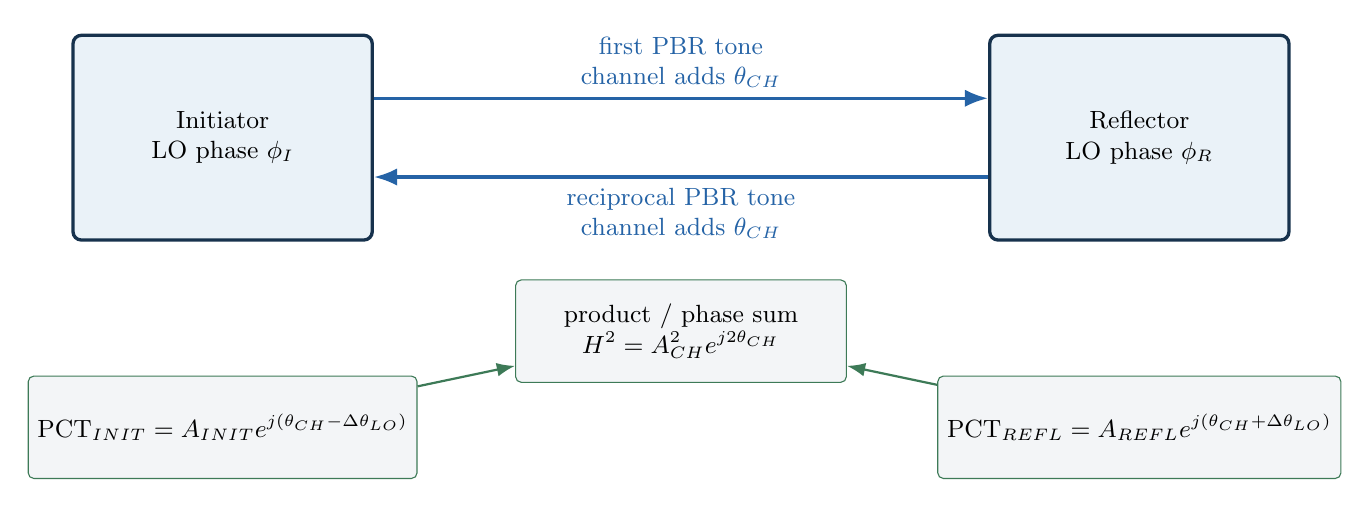
\begin{tikzpicture}[font=\small,>=Latex,node distance=13mm and 23mm]
\tikzset{dev/.style={draw=navy,very thick,rounded corners=3pt,fill=lightblue,minimum width=38mm,minimum height=26mm,align=center}, obs/.style={draw=green,rounded corners=2pt,fill=lightgray,minimum width=42mm,minimum height=13mm,align=center}, ar/.style={-Latex,very thick,color=blue}}
\node[dev] (I) {Initiator\\LO phase $\phi_I$};
\node[dev,right=78mm of I] (R) {Reflector\\LO phase $\phi_R$};
\draw[ar] ($(I.east)+(0,5mm)$)--node[above,align=center]{first PBR tone\\channel adds $\theta_{CH}$} ($(R.west)+(0,5mm)$);
\draw[ar] ($(R.west)+(0,-5mm)$)--node[below,align=center]{reciprocal PBR tone\\channel adds $\theta_{CH}$} ($(I.east)+(0,-5mm)$);
\node[obs,below=17mm of R] (pr) {$\PCT_{REFL}=A_{REFL}e^{j(\theta_{CH}+\Delta\theta_{LO})}$};
\node[obs,below=17mm of I] (pi) {$\PCT_{INIT}=A_{INIT}e^{j(\theta_{CH}-\Delta\theta_{LO})}$};
\node[obs,below=18mm of $(I)!0.5!(R)$] (prod) {product / phase sum\\$H^2=A_{CH}^2e^{j2\theta_{CH}}$};
\draw[-Latex,thick,green] (pr)--(prod);\draw[-Latex,thick,green] (pi)--(prod);
\end{tikzpicture}}
\caption{Conventional reciprocal PCT phase calibration. Static relative LO phase cancels in the product.}
\end{figure}

\subsection{Inline PCT Transfer}
With IPT enabled, the reflector measures its incoming PCT and adjusts the outgoing tone phase in the PHY. The ideal initiator observable is directly
\begin{equation}
\theta_{INIT,IPT}(f)=2\theta_{CH}(f).
\end{equation}
The reflector returns PCT values with zero phase; the real component conveys the defined amplitude and the imaginary component is zero. IPT changes where phase transfer is performed, not the ideal channel-phase observable.

\subsection{LFAE phase correction is not Mode-0 FFO substitution}
Volume 6, Part A, Sec. 6.3 requires a device aware of local frequency actuation error to compensate the phase rotation that error causes between received and transmitted tone centers. In the nominal form,
\begin{equation}
\angle\PCT'=\angle\PCT-2\pi\Delta f_kT_{PM\_CENTER\_DELTA},
\label{eq:lfaephase}
\end{equation}
where $\Delta f_k$ is the local actuation error in hertz and $T_{PM\_CENTER\_DELTA}$ is the relevant antenna-port center separation. Circuit delay and synchronization error may require an implementation-specific correction to the nominal interval.

Part A also states that a device should not compensate a residual frequency error observed during the PCT phase-measurement period except its own LFAE. This is distinct from using Mode-0 FFO for the specified inter-device frequency/timing relationship elsewhere in the CS processing chain.

\subsection{Why residual frequency still matters to PBR}
If a residual frequency error $\delta f$ is carried between two phase references separated by $\Delta t$, the phase error is
\begin{equation}
\delta\phi_{CFO}=2\pi\delta f\Delta t.
\end{equation}
Reciprocal PCT multiplication cancels a static $\Delta\theta_{LO}$ but does not magically remove all time-dependent phase. Correct implementation follows the exact Core correction points: Mode-0 establishes the subevent frequency/timing reference, local LFAE is applied where required, and PCTs represent the specified phase-valid centers.

\section{Complete numerical derivation at 2440 MHz}
\label{sec:example}
Assume step $k$ has
\begin{align*}
f_0[k]&=\SI{2440000000}{\hertz}, & \FAE_R[k]&=-1.5\ \text{ppm},\\
\FFO_{R/I}[k]&=+12\ \text{ppm}, & F_s&=\SI{4}{\mega\sample\per\second},\\
f_{c,cmd}^{(I)}[k]&=f_0[k], & \LFAE_I[k]&=+0.75\ \text{ppm},\\
s_{IQ}&=+1, & T_{obs}&=\SI{80}{\micro\second}.
\end{align*}
The LFAE sign follows Section~\ref{sec:framework}: actual zero-baseband reference minus commanded reference.

\subsection{Remote FAE-adjusted reference and received frequency}
Convert ppm to dimensionless values:
\begin{equation}
a_R=-1.5\times10^{-6},\qquad \eta_{R/I}=12\times10^{-6}.
\end{equation}
Then
\begin{align}
f_{ref,R}&=2,440,000,000(1-1.5\times10^{-6})\\
&=\SI{2439996340}{\hertz},
\end{align}
and the exact received frequency in the initiator coordinate is
\begin{align}
f_{RX}^{(I)}&=f_{ref,R}(1+12\times10^{-6})\\
&=\SI{2440025619.95608}{\hertz}.
\label{eq:examplefrx}
\end{align}

\subsection{Local zero-baseband reference including LFAE}
The local actuation correction in hertz is
\begin{equation}
\delta f_L^{(I)}=2,440,000,000(0.75\times10^{-6})=\SI{1830}{\hertz}.
\end{equation}
Therefore
\begin{equation}
f_c^{(I)}=f_{c,cmd}^{(I)}+\delta f_L^{(I)}
=\SI{2440001830}{\hertz}.
\end{equation}

\subsection{What the I/Q samples contain}
From Eq.~\ref{eq:bbdef},
\begin{align}
\Delta f_{BB}
&=s_{IQ}(f_{RX}^{(I)}-f_c^{(I)})\\
&=+1(2,440,025,619.95608-2,440,001,830)\\
&=\SI{23789.95608}{\hertz}.
\label{eq:examplebb}
\end{align}
At \SI{4}{\mega\sample\per\second},
\begin{equation}
\omega=2\pi\frac{23,789.95608}{4,000,000}
=0.037369\ \text{rad/sample}.
\end{equation}
For the full tone, $N=F_sT_{obs}=320$ and the desired phase advances
\begin{equation}
2\pi\Delta f_{BB}T_{obs}=11.9581\ \text{rad}=1.90320\ \text{cycles}.
\end{equation}

\subsection{Reconstruction from the measured phase rate}
Assume the estimator returns Eq.~\ref{eq:examplebb}. Equation~\ref{eq:freconstructhat} gives
\begin{align}
\widehat f_{RX}^{(I)}
&=2,440,000,000+1,830+23,789.95608\\
&=\SI{2440025619.95608}{\hertz},
\end{align}
which matches Eq.~\ref{eq:examplefrx}.

\subsection{Final FFO}
\begin{align}
\widehat\FFO_{RX}
&=10^6\frac{2,440,025,619.95608-2,439,996,340}{2,439,996,340}\\
&=+12.000000\ \text{ppm}.
\end{align}

Two incorrect shortcuts show why the complete derivation matters.
\begin{itemize}
\item If remote FAE is ignored and $(f_{RX}-f_0)/f_0$ is reported, the result is about +10.5 ppm, not +12 ppm.
\item If the positive local LFAE correction is omitted, the reconstructed frequency is low by \SI{1830}{\hertz} and the FFO result is biased low by approximately 0.750001 ppm.
\end{itemize}

\subsection{Residual frequency translated to phase}
The +12 ppm component relative to $f_{ref,R}$ is \SI{29279.95608}{\hertz}. If left uncompensated across \SI{20}{\micro\second}, it produces
\begin{equation}
2\pi(29,279.95608)(20\times10^{-6})=3.679\ \text{rad}=210.8^\circ.
\end{equation}
This numerical result explains why frequency calibration and phase calibration are separate but coupled requirements.

\clearpage
\section{Error sources, diagnostics, and verification}
\begin{longtable}{@{}p{0.20\linewidth}p{0.25\linewidth}p{0.27\linewidth}p{0.20\linewidth}@{}}
\caption{Representative error budget.}\\
\toprule Source & Mathematical effect & Mitigation & Diagnostic \\
\midrule\endfirsthead
\toprule Source & Mathematical effect & Mitigation & Diagnostic \\
\midrule\endhead
Thermal noise & Random error in $\argp R_m$ or $\theta_n$ & Use valid duration and efficient weighting & Correlation magnitude and repeated variance\\
Phase noise & Correlated $\psi[n]$ & Validate estimator bandwidth & Residual spectrum\\
Within-tone drift & Curvature in phase & Fit curvature or reject transient region & Quadratic phase term\\
RF/AGC settling & Biased early samples & Characterized $t_{settle}$ & Start-index sweep\\
Ramp boundary & Biased late samples & Characterized $t_{tail}$ & End-index sweep\\
DC/LO leakage & Pull toward zero phase rate & Calibrated DC or joint model & DC-to-tone ratio\\
I/Q imbalance & Image tone and phase ripple & Gain/quadrature calibration & Image rejection\\
Sample-rate error & Scales $\widehat{\Delta f}_{BB}$ & Use calibrated $F_s$ & Digital tone injection\\
LFAE sign/value & Additive error in $f_c^{(I)}$ & Declare actual-minus-command sign & Three-point RF test\\
Remote FAE mismatch & Wrong denominator/reference & Use correct channel table entry & Compare table version\\
Alias selection & Adds $qF_s/m$ & Coarse-to-fine estimator & Lag consistency\\
Motion/multipath & Adds $d\phi_{ch}/dt$ & Coherence and residual gates & Window and antenna consistency\\
PCT center error & Phase term $2\pi\delta f\Delta t$ & Use specified valid center & Center-time sweep\\
\bottomrule
\end{longtable}

\subsection{Required verification sequence}
\begin{enumerate}
\item Generate noise-free complex tones and verify Eqs.~\ref{eq:lagproduct}-\ref{eq:dfcorr} over positive and negative frequency.
\item Add known phase noise, DC, I/Q imbalance, clipping, and drift; verify bias and quality gates.
\item Inject a digital tone after downconversion to verify $F_s$, decimation, NCO bookkeeping, and fixed-point scaling.
\item Conducted RF sweep at $f_{ref,R}-\Delta$, $f_{ref,R}$, and $f_{ref,R}+\Delta$ to verify the final sign.
\item Repeat over CS channel, input level, temperature, supply, synchronization PHY, and supported $T_{IP1}$.
\item Use several Mode-0 steps and controlled outliers to verify channel-specific FAE selection and aggregation.
\item Inject known reciprocal PCT phases to verify LO-phase cancellation and the factor of two.
\item Compare IPT enabled and disabled after the prescribed processing; both should yield the same ideal $2\theta_{CH}$ within uncertainty.
\end{enumerate}

\section{Normative behavior versus implementation choice}
\begin{tabularx}{\linewidth}{@{}X X@{}}
\toprule Bluetooth-defined behavior & Implementation-specific design \\
\midrule
Mode-0 exchange order and timing intervals & RF/IF architecture, sample rate, and numeric format\\
Meaning of $f_0$, $f_{RX}$, FAE, LFAE, FFO, and $\FFO_{RX}^{*}$ & Definition of the internal zero-baseband reference and calibration storage\\
Average received tone frequency as the measurement target & Correlation, regression, FFT, maximum-likelihood, or hybrid estimator\\
Use of local actuation error compensation & Sign convention and location of the correction in the receiver chain\\
PCT valid region and LFAE phase correction & Sample weights and quality metrics inside the valid region\\
Reciprocal PCT product and IPT behavior & Hardware phase rotation and internal PCT estimator\\
\bottomrule
\end{tabularx}

\section{Conclusions}
A self-contained Mode-0 implementation requires one declared local frequency coordinate. The reflector transmits a tone whose physical frequency contains its FAE-adjusted reference and its clock-scale error. The initiator observes phase rotation relative to its actual zero-baseband frequency. After converting radians per sample with the calibrated sample rate, it reconstructs $f_{RX}[k]$ by adding the commanded zero frequency, the signed local actuation correction, and the signed baseband residual. Only then is the exact FAE-adjusted Bluetooth FFO equation applied.

The direct result is Eq.~\ref{eq:directffo}, which links measured I/Q correlation phase to $\widehat\FFO_{RX}[k]$ without an unexplained intermediate quantity. The oscillator-frame derivation, Eq.~\ref{eq:exactrelative}, shows why the result is a remote-to-local frequency ratio rather than an absolute laboratory offset. The \SI{2440}{\mega\hertz} example verifies every sign and intermediate value.

Mode-0 frequency/time calibration does not replace Volume 1 phase calibration. Conventional reciprocal PCT multiplication or IPT cancels the static relative LO phase and exposes $2\theta_{CH}$. Correct PBR processing must also use the specified phase-valid centers and the required LFAE phase correction.

\appendix
\section{Compact implementation equations}
For a validated lag-$m$ estimator:
\begin{align}
R_m[k]&=\sum_{n=m}^{N-1}w_nz_k[n]z_k^*[n-m],\\
\widehat{\Delta f}_{BB}[k]&=\frac{F_s}{2\pi m}\left(\argp R_m[k]+2\pi q_k\right),\\
\widehat f_{RX}^{(I)}[k]&=f_{c,cmd}^{(I)}[k]+\widehat{\delta f}_L^{(I)}[k]
+s_{IQ}\widehat{\Delta f}_{BB}[k],\\
\widehat\FFO_{RX}[k]&=10^6\left[
\frac{\widehat f_{RX}^{(I)}[k]}{f_0[k](1+10^{-6}\FAE_R[k])}-1\right]\ \text{ppm}.
\end{align}

These four equations are sufficient only when their symbols follow Section~\ref{sec:framework}, aliases are resolved, $F_s$ is calibrated, and the sample window lies inside $T_{FM}$.

\section{Numerical test vector}
\begin{table}[ht]
\centering
\caption{Deterministic values for the \SI{2440}{\mega\hertz} example.}
\begin{tabularx}{\linewidth}{@{}X r l@{}}
\toprule Quantity & Value & Unit\\\midrule
$f_0$ & 2,440,000,000 & Hz\\
Reflector FAE & -1.5 & ppm\\
$f_{ref,R}$ & 2,439,996,340 & Hz\\
Relative FFO & +12 & ppm\\
$f_{RX}^{(I)}$ & 2,440,025,619.95608 & Hz\\
Commanded zero frequency & 2,440,000,000 & Hz\\
Initiator LFAE & +0.75 & ppm\\
$\delta f_L^{(I)}$ & +1,830 & Hz\\
Actual zero-baseband reference & 2,440,001,830 & Hz\\
$\Delta f_{BB}$ for $s_{IQ}=+1$ & 23,789.95608 & Hz\\
$F_s$ & 4,000,000 & sample/s\\
$N$ over \SI{80}{\micro\second} & 320 & samples\\
Phase increment $\omega$ & 0.037369 & rad/sample\\
Corrected FFO & +12.000000 & ppm\\
\bottomrule
\end{tabularx}
\end{table}

\clearpage
\begin{thebibliography}{9}
\bibitem{arch}
Bluetooth SIG, \emph{Bluetooth Core Specification, Version 6.3}, Vol. 1, Part A, ``Architecture,'' Sec. 9.1 ``Channel Sounding procedure'' and Sec. 9.2 ``Distance estimation based on phase and amplitude information,'' 2026.\\
\url{https://www.bluetooth.com/wp-content/uploads/Files/Specification/HTML/Core_v6.3/out/en/architecture,-change-history,-and-conventions/architecture.html}

\bibitem{phy}
Bluetooth SIG, \emph{Bluetooth Core Specification, Version 6.3}, Vol. 6, Part A, ``Radio Physical Layer Specification,'' Sec. 3.5 ``Frequency measurement and generation in Channel Sounding,'' and Secs. 6.3-6.5, 2026.\\
\url{https://www.bluetooth.com/wp-content/uploads/Files/Specification/HTML/Core_v6.3/out/en/low-energy-controller/radio-physical-layer-specification.html}

\bibitem{cs}
Bluetooth SIG, \emph{Bluetooth Core Specification, Version 6.3}, Vol. 6, Part H, ``Channel Sounding,'' Sec. 4.3.1 ``Channel Sounding step mode-0'' and Sec. 4.6, 2026.\\
\url{https://www.bluetooth.com/wp-content/uploads/Files/Specification/HTML/Core_v6.3/out/en/low-energy-controller/channel-sounding.html}

\bibitem{rfphy}
Bluetooth SIG, \emph{LE Radio Frequency Physical Layer Test Suite}, RFPHY.TS, Sec. 4.8.1 ``CS Step Mode-0, Frequency Verification.''\\
\url{https://files.bluetooth.com/wp-content/uploads/dlm_uploads/2025/11/RFPHY.TS.p24ed2.pdf}

\bibitem{kay}
S. M. Kay, \emph{Fundamentals of Statistical Signal Processing: Estimation Theory}. Prentice Hall, 1993.

\bibitem{quinn}
B. G. Quinn and E. J. Hannan, \emph{The Estimation and Tracking of Frequency}. Cambridge University Press, 2001.
\end{thebibliography}

\end{document}
